%%%%%%%%%%%%%%%%%%%%%%%%%%%%%%%%%%%%%%%%%
% University Assignment Title Page 
% LaTeX Template
% Version 1.0 (27/12/12)
%
% This template has been downloaded from:
% http://www.LaTeXTemplates.com
%
% Original author:
% WikiBooks (http://en.wikibooks.org/wiki/LaTeX/Title_Creation)
%
% License:
% CC BY-NC-SA 3.0 (http://creativecommons.org/licenses/by-nc-sa/3.0/)
% 
% Modified for COSC480/490 by:
% Lech Szymanski (8/3/18)
%
% Modified for Eden's COSC385 report. (09/2025)

\documentclass[12pt]{article}
\usepackage[draft]{cosc4x0style}
\usepackage{float}
\usepackage{tikz}
\usetikzlibrary{shapes,arrows,positioning}

% To compile the final version of the report (which will remove all the todo content)
%\usepackage{cosc4x0style}

% Specify project code 480 or 490
\papercode{385}

% Your project title
\title{Talking in French Like an Academia\\\large Machine Learning Powered Verlan Identification}

% Your name
\author{Yitian \textsc{Li}}
\studentid{4556502}

% Names of your supervisors, separated by line break '\\'
\supervisors{
  Dr. Lech \textsc{Szymanski} \\
  Dr. Veronica \textsc{Liesaputra}
}

% Date, change the \today to a set date if you want to be precise
\reportdate{\today}

\begin{document}


\maketitle

\begin{abstract}
something.
\end{abstract}

\section{Introduction}
\subsection{Context and Motivation}

Since the early 19th century, the French people have started to talk using Verlan. Just like Pig Latin\footnote{\url{en.wikipedia.org/wiki/Pig_Latin}} exists in English culture, Verlan is an unusual and creative form of \textit{argot} (slang) that is formed by flipping the syllables around in a word.\footnote{In fact, the word \textit{Verlan} is a Verlan from the word \textit{l'inver} (the inversion).}\cite{rajabov2025,bach2018} 
Time flies, Verlan has become more and more popular, and it is now widely used amongst teens and young people in francophone societies\footnote{Such as France, Belgium, Switzerland, Luxembourg, and Canada.}\cite{evolutionVerlan}. Examples of Verlan can be as follows:

\begin{flushleft}
\small
\begin{itemize}
  \item bite = bi + te \(\rightarrow\) te + bi \(\rightarrow\) tebie (penis)
  \item shit = shi + t \(\rightarrow\) t + shi \(\rightarrow\) teuchi\cite{evolutionVerlan}
  \item bonjour = bon + jour \(\rightarrow\) jour + bon \(\rightarrow\) jourbon (greetings)
\end{itemize}
\end{flushleft}

\noindent In real-life conversations, such can be used as in the example sentences below:

\begin{flushleft}
\small
\begin{itemize}
  \item \textit{Le graff géant représente une tebie pixel art.}\\(The giant graffiti depicts a pixel art penis.)
  \item \textit{Il a du bon teuchi du bled.}\\(He's got some good shit from the countryside.)
  \item \textit{Un p'tit\footnote{Standard spelling: petit.}jourbon et tout le monde sourit.}\\(A quick hello and everyone smiles.)
\end{itemize}
\end{flushleft}

Indeed, Verlan can be formed with different original languages, not only French, but also English and other languages. However, it always follows the same rule of flipping syllables, although, for better pronunciation reasons, certain minor amendments such as dropping unnecessary letters and applying accents (e.g., é, è) can be used from time to time\cite{rajabov2025}. Besides, due to the universal trait of slang being used more often phonetically instead of written, Verlan users tend to spell them differently when writing them down. As technology develops, this has been occurring more frequently than ever in daily texting\cite{rua2005}.

Thinking internationally, when people are communicating with translators, it is possible that slang in their mother language can be brought to the conversation, which could be tricky for translators to translate\cite{hajiyeva2025}. Using translators such as DeepL\footnote{\url{www.deepl.com}} and Google Translate\footnote{\url{translate.google.com}} to translate sentences that contain Verlan from French to English can be a specific example to prove this. Furthermore, although both of the translators above are using Machine Learning (ML) for translation, their results of translating Verlans are not ideal\cite{deepl2020, wu2016}. For example, when attempting to translate the sentence above, \textit{Le graff géant représente une tebie pixel art.}, both Google Translate\ref{fig:google_Verlan} and DeepL\ref{fig:deepl_Verlan} cannot translate the word \textit{tebie} correctly. Specifically, for DeepL, there is no desired translation as \textit{penis} in its alternative word list for \textit{tebie}\ref{fig:deepl_alt_text}.

\begin{figure}[H]
\centering
\includegraphics[width=0.8\textwidth]{figures/google_Verlan.png}
\caption{\label{fig:google_Verlan}Google Translate cannot translate the Verlan \textit{tebie} correctly.}
\end{figure}

\begin{figure}[H]
\centering
\includegraphics[width=0.8\textwidth]{figures/deepl_Verlan.png}
\caption{\label{fig:deepl_Verlan}DeepL cannot translate the Verlan \textit{tebie} correctly.}
\end{figure}

\begin{figure}[H]
\centering
\includegraphics[width=0.3\textwidth]{figures/deepl_alt_text.png}
\caption{\label{fig:deepl_alt_text}No desired translation for Verlan \textit{tebie} in DeepL's alternative word list.}
\end{figure}

Thus, a question shall naturally arise: Can we improve translators' performance in translating slang by improving the ML model? The answer is undoubtedly `yes' in an era where artificial intelligence research is expanding rapidly. Researchers have been making progress in identifying slang using ML\cite{pei2019slang} and, moreover, in translating noisy text, of which slang is a part\cite{michel2018mtnt}. 

But what about Verlan? There is no known ongoing or completed research on identifying \textit{such} slang or their translations\footnote{Until September 2025.}, nor does a proper dataset exist. The only work similar to this is an assignment published at the University of Toronto\footnote{\url{https://uoft-csc413.github.io/2022/assets/assignments/PA03.pdf}}, asking students to train a Neural Machine Translation (NMT) model to transform standard English into Pig Latin. It is not only the other way around; instead of identifying Pig Latin and transforming it back to standard English, it is also more of an example for students to practice using NMT than a discussion on its identification and translation. Shouldn't we do something?

This report aims to change that.

\subsection{Objective}

The purpose of the project is to create two Verlan datasets: one functioning as a dictionary, containing the Verlan words and their normalised standard French equivalents; the other a dataset of sentences that contain Verlan, paired with the same sentences containing normalised words, with labels indicating whether a sentence contains Verlan. After that, the project embeds and classifies Verlan using Large Language Models (LLMs) and analyses the results.

\begin{figure}[H]
\centering
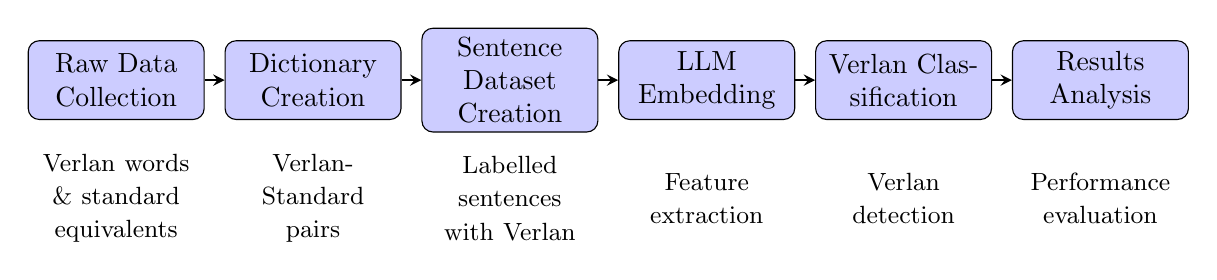
\begin{tikzpicture}[
    node distance=2.5cm,
    auto,
    block/.style={rectangle, draw, fill=blue!20, text width=2cm, text centered, rounded corners, minimum height=1cm},
    arrow/.style={thick,->,>=stealth}
]

% Define nodes from left to right
\node [block] (data) {Raw Data Collection};
\node [block, right of=data] (dict) {Dictionary Creation};
\node [block, right of=dict] (sentences) {Sentence Dataset Creation};
\node [block, right of=sentences] (embedding) {LLM Embedding};
\node [block, right of=embedding] (classification) {Verlan Classification};
\node [block, right of=classification] (analysis) {Results Analysis};

% Draw arrows
\draw [arrow] (data) -- (dict);
\draw [arrow] (dict) -- (sentences);
\draw [arrow] (sentences) -- (embedding);
\draw [arrow] (embedding) -- (classification);
\draw [arrow] (classification) -- (analysis);

% Add labels below nodes
\node [below of=data, node distance=1.5cm, text width=2cm, text centered] {\small Verlan words \& standard equivalents};
\node [below of=dict, node distance=1.5cm, text width=2cm, text centered] {\small Verlan-Standard pairs};
\node [below of=sentences, node distance=1.5cm, text width=2cm, text centered] {\small Labelled sentences with Verlan};
\node [below of=embedding, node distance=1.5cm, text width=2cm, text centered] {\small Feature extraction};
\node [below of=classification, node distance=1.5cm, text width=2cm, text centered] {\small Verlan detection};
\node [below of=analysis, node distance=1.5cm, text width=2cm, text centered] {\small Performance evaluation};

\end{tikzpicture}
\caption{\label{fig:pipeline}A visulisation of the objectives.}
\end{figure}

With the purpose above, the report contributes to the linguistics and the AI researchers two Verlan datasets, for dictionary making or LLMs training. The report also evaluates how good we can achieve the identification of Verlan with ML, to benefit machine translation in the future.

The code and the unannotated, un peer-reviewed dataset developed as part of the project are released under openlicences and aligns with open science best practices, with the usage of a version controlled software development platform (GitHub)\footnote{\url{github.com/greateden/Verlan-Identification-Normalisation}}. The annotated, peer-reviewed dataset will be published shortly after this report, aiming by the end of 2025.

\section{Background}
\subsection{How Francophone People Use Verlan}
This section is to help those readers who don't have a linguistic backgound in Verlan to clean their fogs.
TODO 
ref the Paris VIII thesis.
mention academie francaise.


\subsection{How to Detect Verlan}

To the best of our knowledge, there is no existing computational research\footnote{As of September 2025.} on the \textit{detection} of Verlan\;---\;this particular form of French slang. However, there are a few scholars who included Verlan in their research\cite{zurbuchen2024, podhorna2020rapcor, mekki2021tremolo, panckhurst202088milsms}. Yet, these research commonly included Verlan as a type of slang in their dataset or corpus. Moreover, they did not extract and research on how to detect this specific type of slang, but in a broader way\;---\;they create slang datasets which contain Verlan, and some of them used computational approaches to detect those slang. 

Luckily, there are quite a few papers related to computational slang detection, and their approaches could contribute to Verlan detection to a large extent\cite{pei2019slang, sun2024informal, slangornot2024, wu2018slangsd}, which are not limited to French, but also cover other Indo-European languages\footnote{For example, English, German, and Russian. For more information, please refer to: \url{https://en.wikipedia.org/wiki/Indo-European_languages}.}.

Therefore, regarding the history of Verlan detection, this report firstly generalises the task as slang detection, constructed based on a slang detection paper's background chapter\cite{pei2019slang}. After each key historical point, there will be discussions related to theoretical ways to implement those methods for Verlan detection, in order to provide the readers with a general and useful background.


\subsubsection{Dictionary Search}
The easiest way we can think of is to use a dictionary, or a corpus --- just like how we look up a word that we don't know of. The pros and cons are just like using a dictionary. It is fast (if using a computer) and accurate. On the other hand, the resource is limited, and it only works with those words which already existed, thus it cannot identify newly invented words. The existing works for slang glossaries are, for example, This is

\subsubsection{Traditional ML}



% Besides, identifying the same word with different spelling or declensions is also a hurdle.






\section{\LaTeX{} markup examples}
\label{sec:examples}
 
\subsection{Sections}

Use \verb$\section{}$ and \verb$subsection{}$ commands to organise your document. \LaTeX{} handles all the formatting and numbering automatically. Use \verb$\label{}$ and \verb$\ref{}$ commands for cross-references.

\subsection{Comments}

Comments might be useful during the writing process, as reminders or questions to your supervisor (who should get a chance to comment on your report). Comments can be added to the margins of the document using the \todo{Here's a comment in the margin!} \verb$\todo{}$ command, as shown in the example on the right. You can also add inline comments:

\todo[inline, color=green!40]{This is an inline comment.}

\subsection{Tables and Figures}

Use the \verb$table{}$ and \verb$\tabular{}$ commands for basic tables --- see Table~\ref{tab:widgets}, for example. You can include a figure (JPEG, PNG or PDF) with the \verb$\includegraphics{}$ command as in the code for Figure~\ref{fig:frog} below.


\begin{table}
\centering
\begin{tabular}{l|r}
Item & Quantity \\\hline
Widgets & 42 \\
Gadgets & 13
\end{tabular}
\caption{\label{tab:widgets}An example table.}
\end{table}

\subsection{Mathematics}

\LaTeX{} is great at typesetting mathematics. Let $X_1, X_2, \ldots, X_n$ be a sequence of independent and identically distributed random variables with $\text{E}[X_i] = \mu$ and $\text{Var}[X_i] = \sigma^2 < \infty$, and let
\begin{equation}S_n = \frac{X_1 + X_2 + \cdots + X_n}{n}
      = \frac{1}{n}\sum_{i}^{n} X_i\label{my_eq1}\end{equation}
denote their mean. Then as $n$ approaches infinity, the random variables $\sqrt{n}(S_n - \mu)$ converge in distribution to a normal $\mathcal{N}(0, \sigma^2)$. You can also reference labeled equations, such as Equation~\ref{my_eq1}.

\subsection{Lists}

You can make lists with automatic numbering \dots

\begin{enumerate}
\item Like this,
\item and like this.
\end{enumerate}
\dots or bullet points \dots
\begin{itemize}
\item Like this,
\item and like this.
\end{itemize}

\section{Conclusion}

Concluding remarks. Send the pdf (not the \verb$*.tex$ file) to your supervisor for comments (as early as possible). Don't forget to change the\\ \verb$\usepackage[draft]{cosc4x0style}$ setting to\\ \verb$\usepackage{cosc4x0style}$ to produce the pdf in the format for the final submission.

%The environment \thebibliography produces a list of references; such list will be titled "References". A parameter inside braces, 9 in the example, indicates the number of entries to be added; this parameter can not be greater than 99.

%To create a bibliography entry the command \bibitem is used. A parameter inside braces is set to label this entry and can later be used as identifier for this reference. After the closing brace the text with the name of the author, the book title, publisher and so on is entered. 

%Any choice of citation style is acceptable as long as you are consistent.

\begin{thebibliography}{9}

\bibitem{rajabov2025} 
Radjabov, Ruslan Rajabmurodovich. \textit{Understanding "Verlan" in the French Language}. 
Web of Scientist: International Scientific Research Journal, vol. 6, no. 3, 2025, pp. 368–372. 
Available at: \url{https://webofjournals.com/index.php/3/article/view/3264}.

\bibitem{bach2018} 
Bach, Xavier. \textit{Tracing the origins of Verlan in an early nineteenth century text}. 
Journal of French Language Studies, vol. 28, no. 1, 2018, pp. 1–18. 
Cambridge University Press. doi:10.1017/S0959269516000221.

\bibitem{evolutionVerlan} 
Olivier Sécardin. \textit{Évolution du Verlan, marqueur social et identitaire, comme reflet de la langue et de la société françaises}. 
Synergies Europe, no. 3, 2008, pp. 223–232. 
Available at: \url{https://journal.lib.uoguelph.ca/index.php/synergies/article/download/1037/1859?inline=1}.

\bibitem{rua2005} 
Rúa, Paula López. “Shortening Devices in Text Messaging.” 
\textit{Journal of Computer-Mediated Communication}, vol. 10, no. 4, July 2005. 
Wiley. doi:10.1111/j.1083-6101.2005.tb00268.x.

\bibitem{hajiyeva2025}  
Hajiyeva, Bulbul. “Translating Idioms and Slang: Problems, Strategies, and Cultural Implications.”  
Acta Globalis Humanitatis et Linguarum, vol. 2, no. 2, 2025, pp. 284–293. doi:10.69760/aghel.025002123.  

\bibitem{deepl2020} 
DeepL. “DeepL Translator translates texts using artificial neural networks. These networks are trained on many millions of translated texts.” 
\textit{DeepL Blog}, 2020. Available at: \url{https://www.deepl.com/en/blog/how-does-deepl-work}.

\bibitem{wu2016} 
Wu, Yonghui, et al. “Google’s Neural Machine Translation System: Bridging the Gap between Human and Machine Translation.” 
arXiv preprint arXiv:1609.08144, 2016. Available at: \url{https://arxiv.org/abs/1609.08144}.

\bibitem{michel2018mtnt}
Michel, Paul, and Graham Neubig. “MTNT: A Testbed for Machine Translation of Noisy Text.”
\textit{Proceedings of EMNLP}, 2018. Available at: \url{https://aclanthology.org/D18-1050/}.

\bibitem{zurbuchen2024}
Zurbuchen, Lucas, and Rob Voigt.  
\textit{A Computational Analysis and Exploration of Linguistic Borrowings in French Rap Lyrics}.  
In *Proceedings of the 62nd Annual Meeting of the Association for Computational Linguistics — Student Research Workshop (ACL SRW 2024)*, 2024, pp. 200–208.  
DOI: 10.18653/v1/2024.acl-srw.27.  
Available at: \url{https://aclanthology.org/2024.acl-srw.27/}.

\bibitem{podhorna2020rapcor}
Podhorná-Polická, Alena.  
\textit{RapCor, Francophone Rap Songs Text Corpus}.  
In *Proceedings of the Fourteenth Workshop on Recent Advances in Slavonic Natural Language Processing (RASLAN 2020)*, 2020, pp. 95–102.  
Available at: \url{https://nlp.fi.muni.cz/raslan/raslan20.pdf#page=95}.  % (no DOI found)

\bibitem{mekki2021tremolo}
Mekki, Jade; Lecorvé, Gwénolé; Battistelli, Delphine; Béchet, Nicolas.  
\textit{TREMoLo-Tweets: A Multi-Label Corpus of French Tweets for Language Register Characterization}.  
In *Proceedings of the International Conference on Recent Advances in Natural Language Processing (RANLP 2021)*, Held Online, INCOMA Ltd., Sep 1–3, 2021, pp. 950–958.  
DOI: 10.26615/978-954-452-072-4\_108.  
Available at: \url{https://aclanthology.org/2021.ranlp-1.108/}.

\bibitem{panckhurst202088milsms}
Panckhurst, Rachel; Lopez, Cédric; Roche, Mathieu.  
\textit{A French text-message corpus: 88milSMS. Synthesis and usage}.  
Corpus [En ligne], 20 | 2020 (mis en ligne le 28 janvier 2020).  
DOI: 10.4000/corpus.4852.  
Available at: \url{https://journals.openedition.org/corpus/4852}.

\bibitem{pei2019slang}
Pei, Zhengqi, Zhewei Sun, and Yang Xu.  
\textit{Slang Detection and Identification}.  
In *Proceedings of the 23rd Conference on Computational Natural Language Learning (CoNLL 2019)*, Hong Kong, China, 2019, pp. 881–889.  
Available at: \url{https://aclanthology.org/K19-1082/}.  % (ACL Anthology entry — no DOI)

\bibitem{sun2024informal}
Sun, Zhewei, Qian Hu, et al.  
\textit{Toward Informal Language Processing: Knowledge of Slang in Large Language Models}.  
In *Proceedings of the 2024 Conference of the North American Chapter of the Association for Computational Linguistics (NAACL 2024)*, 2024.  
DOI: 10.18653/v1/2024.naacl-long.94.  
Available at: \url{https://aclanthology.org/2024.naacl-long.94/}.

\bibitem{slangornot2024}
Anonymous.  
\textit{Slang or Not? Exploring NLP Techniques for Slang Detection Using the SlangTrack Dataset}.  
ACL ARR (OpenReview) submission, December 2024 (ACL ARR 2024 December).  
Available at: \url{https://openreview.net/forum?id=bISO3DD8sU}.

\bibitem{wu2018slangsd}
Wu, Tianyang; Morstatter, Fred; Liu, Huan; et al.  
\textit{SlangSD: Building, Expanding, and Using a Sentiment Dictionary of Slang Words for Short-Text Sentiment Classification}.  
Language Resources and Evaluation (2018).  
DOI: 10.1007/s10579-018-9416-0.  
Available at: \url{https://link.springer.com/article/10.1007/s10579-018-9416-0}.



\end{thebibliography}


% Activate the appendix
% from now on sections are numerated with capital letters
\appendix

\renewcommand{\thesection}{Appendix \Alph{section}}

\section{Some extra things}

If you have anything more to add such as:
\begin{itemize}
\item not essential details - things that might be too much for first time reading, or could be distracting from the main points...but are still important for reproducibility or deeper understanding
\item work that was done in the project but doesn't go with the main work, or detracts/is not essential for the main narrative.  
\end{itemize}

\section{Aims and Objectives}

\textbf{Interim report only!} -- you do not need to include this appendix in the final report.  However, in your interim the last appendix should include your original Aims and Objectives, and, if the things have changed, the revised Aims and Objectives. If you used the \LaTeX{} template provided for your Aims and objectives document, just copy the \verb$\paragraph{Aims}$ and \verb$\paragraph{Objectives}$ sections and paste them here.

\subsection*{Original}

\paragraph{Aims}
Here you are describing the term goal of the project. What do you want to achieve by the end?  What is the ultimate goal of this work?  For example, the primary aim of this document is to have students produce suitable aims and objectives for their COSC480/490 project. While the aims and objectives document is not an assessed deliverable, a clear definition of what is to be done, and a bit of planning of how it is to be accomplished is paramount to the project's success. It is important to establish the scope of the project.

\paragraph{Objectives}
Objectives list the milestones that you need to achieve in order to achieve the projects aim(s). It's a rough plan for what needs to happen in what order. It's best to list the objectives in bullet point form. For many projects the structure to these objectives might follow the following pattern (objective names are just examples -- you can have different objective names):    
\begin{itemize}[noitemsep]
\item background reading; going through the literature; learning about the research field;
\item setting up of some kind of system for the project; getting the environment for experiments working;
\item conducting preliminary experiments; implementation of a basic/simple approach; producing base case results;
\item trying method 1; recording the results;
\item trying method 2; recording the results.
\end{itemize}

\subsection*{Revised}

\paragraph{Aims}
Here you are describing the term goal of the project. What do you want to achieve by the end?  What is the ultimate goal of this work?  For example, the primary aim of this document is to have students produce suitable aims and objectives for their COSC480/490 project. While the aims and objectives document is not an assessed deliverable, a clear definition of what is to be done, and a bit of planning of how it is to be accomplished is paramount to the project's success. It is important to establish the scope of the project.

\paragraph{Objectives}
Objectives list the milestones that you need to achieve in order to achieve the projects aim(s). It's a rough plan for what needs to happen in what order. It's best to list the objectives in bullet point form. For many projects the structure to these objectives might follow the following pattern (objective names are just examples -- you can have different objective names):    
\begin{itemize}[noitemsep]
\item background reading; going through the literature; learning about the research field;
\item setting up of some kind of system for the project; getting the environment for experiments working;
\item conducting preliminary experiments; implementation of a basic/simple approach; producing base case results;
\item trying method 1; recording the results;
\item trying method 2; recording the results.
\end{itemize}


\end{document}